\documentclass[conference,12pt]{IEEEtran}
\usepackage{pdflscape}
\usepackage{longtable}
\usepackage[bitheight=6ex]{bytefield}
\usepackage{todonotes}
\usepackage{hyperref}
\usepackage{tabularx}
\usepackage{graphicx, subfigure, amsmath} 
\usepackage{pdfpages}
\usepackage[backend=biber,style=ieee]{biblatex}
%\usepackage[section]{placeins}
\addbibresource{References.bib}
\interdisplaylinepenalty=2500

% correct bad hyphenation here
\hyphenation{}


\begin{document}
%
% paper title
\title{Automotive Communications \\ \large{Better Than Best Effort}}

\author{
\IEEEauthorblockN{Jeremy Wright}
\IEEEauthorblockA{Arizona State University\\jlwrigh1@asu.edu}
}
\maketitle
\begin{abstract}
Vehicle's are quickly becoming distributed comupting platforms on wheels, and
teh integration of these system is essentail for both the safety and comfort of
the passengers. Over the last few decades there has been increasing integrtion
of these systems to perform highly advanced functions, but never losing thier
core safety and realibility guiarntees. This survey will look at the 4 most
popular industial networks in vehciles, how they differ from the enthernet based
protocols we are used to in the internet domain, and how the physical layers and
software layers interact to make a truely safe system. 
\end{abstract}

\begin{IEEEkeywords}
CAN, LIN, MOST, FlexRay, safety, reliability
\end{IEEEkeywords}

\section{Introduction}

Something flashes across the road. Instinctively you slam on the brakes. ABS
kicks in to preserve tire contact with the road. Your body begins to fly
forward, your head towards the steering wheel. Inertial sensors deploy a series
of events collision management events. The fuel pump is shut down to reduce the
risk of fire. Body dynamic sensors adjust suspension forces to keep the vehicle
level, and in a safe driving position. The vehicle signals emergency responders
of a crash event with the current GPS location. You are caught by the air bag.
The crash is over. You are safe. 

This is the environment of automotive networks.
The hard real-time communication channels where failure means people die.
Advances made in this area have increased vehicle safety, reduced vehicle
weight, and improved overall comfort of the system \autocite{navet_trends_2005}. Many of us are familiar with
Internet application network Ethernet, and its approach to security. Network
security is defined by 4 principles: Confidentiality, Integrity, Availability,
and non-repudiation.   Ethernet attempts to meet a centroid by spreading
responsibilities across the various layers of the protocol. Automotive networks
however choose to optimize just two of these aspects, Availability, and Integrity.
Messages must be able to be send when ready, and message must arrive intact.

Internet protocol is fault
tolerant and employs a concept called best effort routing, where packets are
routed to a destination in the most likely path for success.  Packets have
a time to live, and if they don't reach the destination in time, drop off the
network \autocite{_best-effort_2014}. Consider since a ``best effort'' approach in a vehicle. 
If the music
player is shipping data over the vehicle network, and the air bag deploy message
cannot get any bandwidth catastrophe. Instead of best effort, industrial
protocols take a different approach focused on safety, reliability, and
guaranteed delivery. This focus usually is a trade-off for performance.  You may
not be able to ship a great deal of data, but what data can be sent is sent
reliability since, when the air bag needs to deploy, being late is useless.

This survey will discuss the industrial physical layers commonly used in
vehicles today: CAN \autocite{std_can}, LIN \autocite{std_lin} and FlexRay
\autcite{std_flexray}, and the software protocols that run over
them, ISO, FlexRay, and MOST. Vehicle network design takes an approach similar
to a VoIP network than how one would design a network primarily for email, and
internet.  In these types of networks latency and jitter are key functions that
translate to real physical requirements. This is typically dealt with in
2 methods Time-Triggered messaged, and Priority Messages. Time Triggered
messages are used when the physical later does not support priority based voting,
where as   in the case of CAN, the physical open-collector function implements
a primitive, yet very effective voting scheme for sending data. This survey will
discuss how messages are segregated into time trigger, or priority networks.
The 4 types of networks running in the vehicle: comfort, chassis, engine, and
describe how these functions work together to provide an immersive infotainment
experience, while keeping our vehicles safer than ever.  

Vehicle functions are
segregated into discrete Electronic Control Units (ECUs) distributed around the
vehicle. These ECUs provide raw sensor data, engine statistics, trouble code
information, and even dynamic suspension information, all in real-time. Before
the advent of CAN in 1986, these systems were completely segregated, and often
implemented by different vendors e.g. the door lock system would be physically
separated from the truck latch.  Segregated there was no issue of contention
since the system fully owned the communication channels it needed. hwever this
also resulted in a great deal of redundency, cost, and weight \todo{cite bmw
weight}.  Furthermore, many functions can have enhancled accuracy or precision
by combining several different data sources in a scheme called sensor fusion.
CAN was intrduced to address these issues.  CAN allowed ECUs to be linked
together with a single twisted pair of copper wires, and included a novel
prioirty scheme for routing higher prioirty messages ahead of lower porioty
ones. This was the advent of the industrial protocol in automotive vehciles.

one level of abstraction above the ECU are the system categories: powertrain,
comfort, and chassis.  powertrain systems involve engine and transmission
data, and have the very tight timing, and jitter specification since these
systems are responsible for function such as variable valve timing, spark
advance/delay and other critical engine functions. comfort is the other end of
the spectrum, and provides the environment controls such as AC, heating, and
radio.  Increasingly these comfort systems have grown to include cellular phone
integration, and even hotspot functionality. This network categroy requires
higher bandwidth, and higher speed but with a lower enphasis on safety, and
reliability. Late message may disrupt the music, but it will not likely result
in harm.  Chassis systems are responsible for maintaining control of suspension,
steering and braking. These are a high reliability network type.
\autocite{navet_trends_2005}.


Industrial protocols allow networked ECUs to
communicate in our vehicles, and airplanes. Protocols such as CAN, LIN, or AFDX,
and their associated physical layers CAN, UART, Ethernet allow for reliable,
scalable, and safe operation of electronic systems within our vehicles.  But
what is it that separates an industrial protocol from a non-industrial one.
Namely, reliability, and safety.  Industrial protocols can be evaluated in how
they meet criteria related to confirmed delivery.  Industrial protocols
typically reduce the bandwidth and speed of the network to add extra
reliability. For instance, CAN uses an open collector signaling scheme which
increases the power required to drive the network than the magnetic isolation
technique of Ethernet, but this simple fact implements an OR operation. This OR
operation is used by senders to verify that each bit they send was received by
the rest of the network.  

CAN was the first industrial protocol introduced by
Bosch in 1983 \autocite{std_can}. Software assisted vehicle functions were connected by point to
point wiring.  Once CAN allowed multiple ECUs to be reliably connected on
a common pair of wires, vehicle manufactures saw improved reliability and
reduced vehicle weight \autocite{navet_trends_2005}.  Industrial portals also allow ECUs to
work cooperatively merging sensor data from multiple end points to achieve
advanced vehicle functions. Today, the X-by-wire systems are the epitome of this
capable of detecting road obstructions and even stopping the vehicle if
necessary.  

So how is reliability defined? Withing vehciles, reliability maps to the
security concept of availability. The message bus must be available when a high
prioiy message is to be sent, and the latency must be abslutely bounded.
Furthermore vehicles are electrically very harsh environments. Temperatures can
be extreme, sensors, and system are exposed to weather. Because of this the
physical layers must continue to function in the presense of high electric
fields or magnetice fields or other anomouly.  Ethernet for example doesn't meet
this requirement. Within HVAC, one must be carefy to lay ethernet lines around
flourcent tube lighting. The magnetic fields genertaed by the neon gasses
arching can disrupt the ethernet cables high higher speeds. In a vehcile this
variably of network quality is unacceptable. 


\section{Reliable Networks}
Reliability is an ECU knowing that
a message sent was received by its intended receiver. Real-time. Vehicle busses
must allow message to arrive in a deterministic amount of time. Since message
could contain life critical message such as �deploy air bags� such highest
priority message must get through. This is also related to safety, at the
protocol level, message must get though, at the signal level vehicles are
electrically very noisy. Noise can induce eddy currently or other anomalous bits
in the digital networks. The physical layer must protect against these to
achieve safe operation.  This survey will look at 4 ground based vehicle
industrial protocols, CAN, LIN, and FlexRay examine the network and
physical layers to how they achieve safety, reliability, data integrity and some
of the security implications of each. Lastly we will look at time triggered,
verses event triggered message schemes an how each system fits into the overal
safety case. 

Besides relability networks provide different levels of performance separated by
their class.
\begin{table}[!t]
\renewcommand{\arraystretch}{1.3}
\caption{Network Classes by speed}
\label{tbl:network_classes}
\centering
\begin{tabular}{c c c}
\hline
\bfseries Network Class & \bfseries Speed & \bfseries Typical Use \\ \hline
\hline
A & $< 10$ Kbps  & Body domain \\
B & $< 125$ Kbps & Sensor Sharing \\
C & $< 1$ Mbps   & Powertrain and Chassis Domain \\
D & $> 1$ Mbps    & Media and infotainment \\
\hline
\end{tabular}
\end{table}

\subsection{CAN} 
CAN is a Class C, half-duplex, self-initated network type. CAN provides prioity based messaging by
implementing an OR function into the physical layer itself. 


\begin{figure}
  \centering
  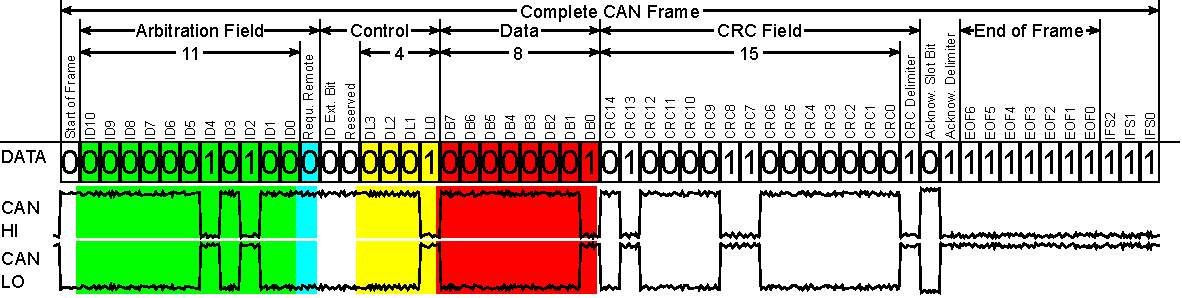
\includegraphics[width=0.4\textwidth]{can_frame.pdf}
  \caption{CAN Frame without bit stuffing}
  \label{fig:can_frame}
\end{figure}
Can was the first industrial protocol for vehicles, and CAN is used for nearly
all systems of a vehicle, except for the comfort system which require higher
bandwidth than CAN provides. The novel concept introduced by CAN was the bit
priority voting system built into the FlexRay Flexray did some stuff that some
people care about, do I care, probably not, but whatev.

\todo{Show network packet structure}
\todo{Show how the voting/priority works}
\todo{describe now the internal hardware provides and additional level of
priority}

\subsection{LIN}
LIN is a class A, half duplex, master initiated network type. It provides a low cost network capable of
interfacing up to 16 separate slave units. LIN is a half-
\begin{figure}
  \centering
  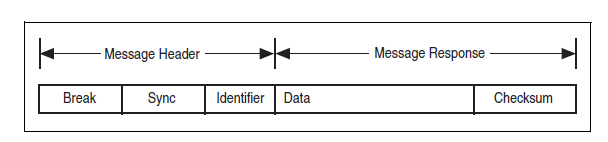
\includegraphics[width=0.4\textwidth]{LIN_frame.png}
  \caption{LIN frame}
  \label{fig:lin_frame}
\end{figure}
\todo{network topography}
\todo{How it acheives guarnateed latency}
Lin bus is a serial bus designed for ultra-low cost low data rate systems.

\subsection{Flexray}
FlexRay is a Class D, full duplex self initiated, network type. It provides very high performance up to 10
Mbps while retaining a strong transmission error correctino scheme.  
\begin{figure}
  \centering
  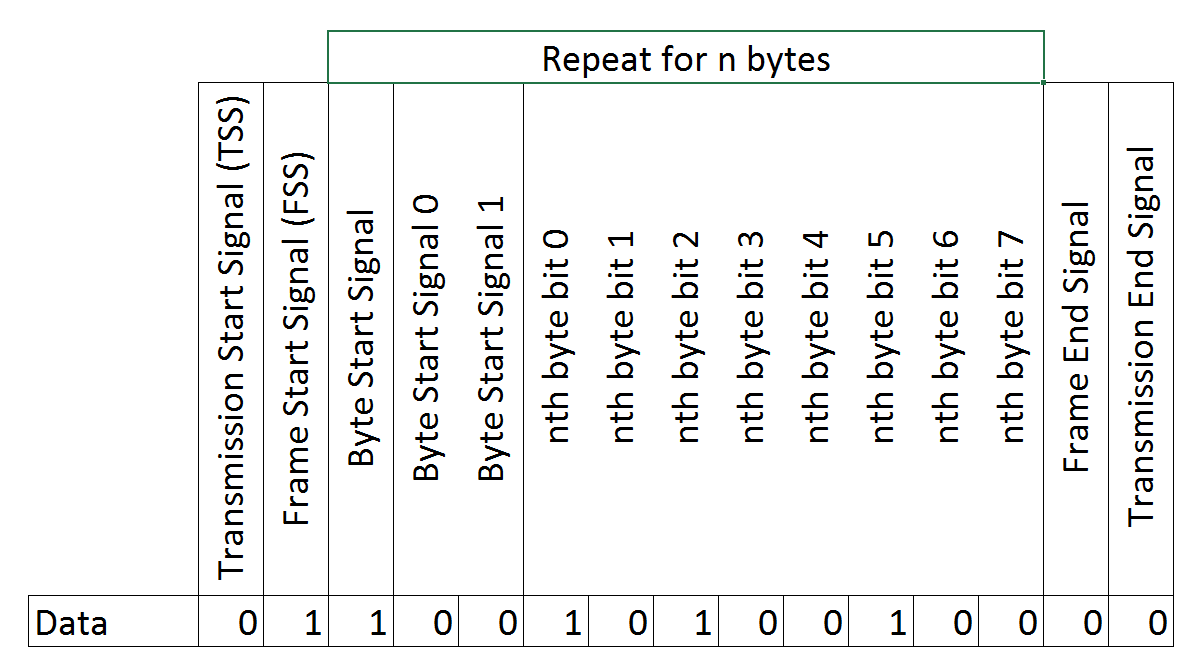
\includegraphics[width=0.4\textwidth]{Flexray.PNG}
  \caption{FlexRay frame}
  \label{fig:flexray_frame}
\end{figure}

\section{Messaging Schemes}
Each of the network types we've looked at are single media, multiple access
networks.  All ECUs, share a single set of wires to communicate to each other.
Ethernet is also such a configuration. However Ethernet's start of transmission
scheme is in start contract to industrial protocls presented here. Ethernet has
a randomized backoff scheme which manaifest a variable network latency scheme.
If a device is a very loud talker, it can push out all other communication
creating a classic denial of service. In a vehcile bus, denial of service, i.e.
the steering wheel cannot contact the power steering unit as in a steer-by-wire
system. Such an event renders the vehcile an uncontrollable missle. But where Ethernet has variable latency
due to its randomized start of transmission scheme, industrial protocols have
two major schemes time triggered, and event triggered messaging for dealing with denial of service, and define a fixed
latency. 
\subsection{Time Triggered Messages}
Time triggered message schemes send data at a rated defined by a network
``master schedule''. This is essentially time division multiplexing the
communication channel. The upseide to time triggered messaging is the simplicy
of analysis. When all messages are defined for bounded windows of transmission,
it is excplicitly known what all message latencies are.  The downside is
composability. Vehicle manufactures tend to build vehicle systems over time,
making small improvements and composing new functions reusing smaller functions
which already exist. Since the ``master schedule'', is truly a single document
describing all traffic, adding a new ECU to the network requires the entire
schedule to be redesigned and evaluated. 

Time triggered messaging is primarily used in fail-safe systems such as steering
and braking. BMW's steer-by-wire systems use FlexRay for very high speed
communication, between the steering wheel, and the steering actuators. The
steering wheel sends it's current angle, and velocity periodically to the
actuator. If the actuator doesn't recieve a message from the steering wheel on
the scheduled time, it can perform some error mechanism to protect the vehcile
from a potentially failed steering wheel.  Braking is a similar design allowing
the vehicle to fail safely if communication channels are faulty. 

\subsection{Event Triggered Messages}
Event triggered schemes preserve bandwidth over time triggered schemes since
ECUs are not sending repeat messages at defined rates. This allows lower speed
busses such as Low speed CAN (125Kbps) to more efficiently use the
limited perforamnce. This however can make the latency more difficult to reason
about. If the message schema does not support priority, then its possible for
lower priorty messages to flood the bus, and prevent higher piroity messages
from reaching the destination before the deadline. 

\section{Conclusion}
Vehicle electronic are trending toward higher connectivity, higher security, and
greater integration within the vehcile as well as new out of vehicle systems.
These trends are already pushing the performance limits of its backbone protcol
CAN, and while MOST provides a higher bandwidth link, it cannot complete with
the safety offered by CAN. It is an exciting time to see what advanced will be
made in the realm of vehcile protocols to meet this growing bandwith bottleneck,
but maintain the critical safety specifications which keeps us blissfully unaware
of the mountain of software that make our cars function. 

\printbibliography

\end{document}
